\documentclass[conference]{IEEEtran}
\IEEEoverridecommandlockouts
% The preceding line is only needed to identify funding in the first footnote. If that is unneeded, please comment it out.
\usepackage{cite}
\usepackage{amsmath,amssymb,amsfonts}
\usepackage{graphicx}
\usepackage{textcomp}
\usepackage{xcolor}
\def\BibTeX{{\rm B\kern-.05em{\sc i\kern-.025em b}\kern-.08em
    T\kern-.1667em\lower.7ex\hbox{E}\kern-.125emX}}
\title{
\vspace{1cm}
{
\includegraphics[width=0.15\textwidth]{iithlogo.jpg } \\ Arm Assignment} }
\author{Ruchika Akkugari\\ Roll No: FWC22276\\ akkugariruchika@gmail.com}
 \begin{document}
\maketitle
 \section {ABSTRACT}
 The objective is to implement and verify a Boolean function simplification using arm through vaman board. The given Boolean function,$F(P,Q,R,S)=\bar{P}\bar{Q}+\bar{P}QS+P\bar{QRS}+P\bar{Q}R\bar{S}$ is simplified to $\bar{PQ}+\bar{QS}$
 implementation uses a vaman board to demonstrate the function’s behavior through hardware configuration and code.
 \begin{figure}[h]
	 \centering
	 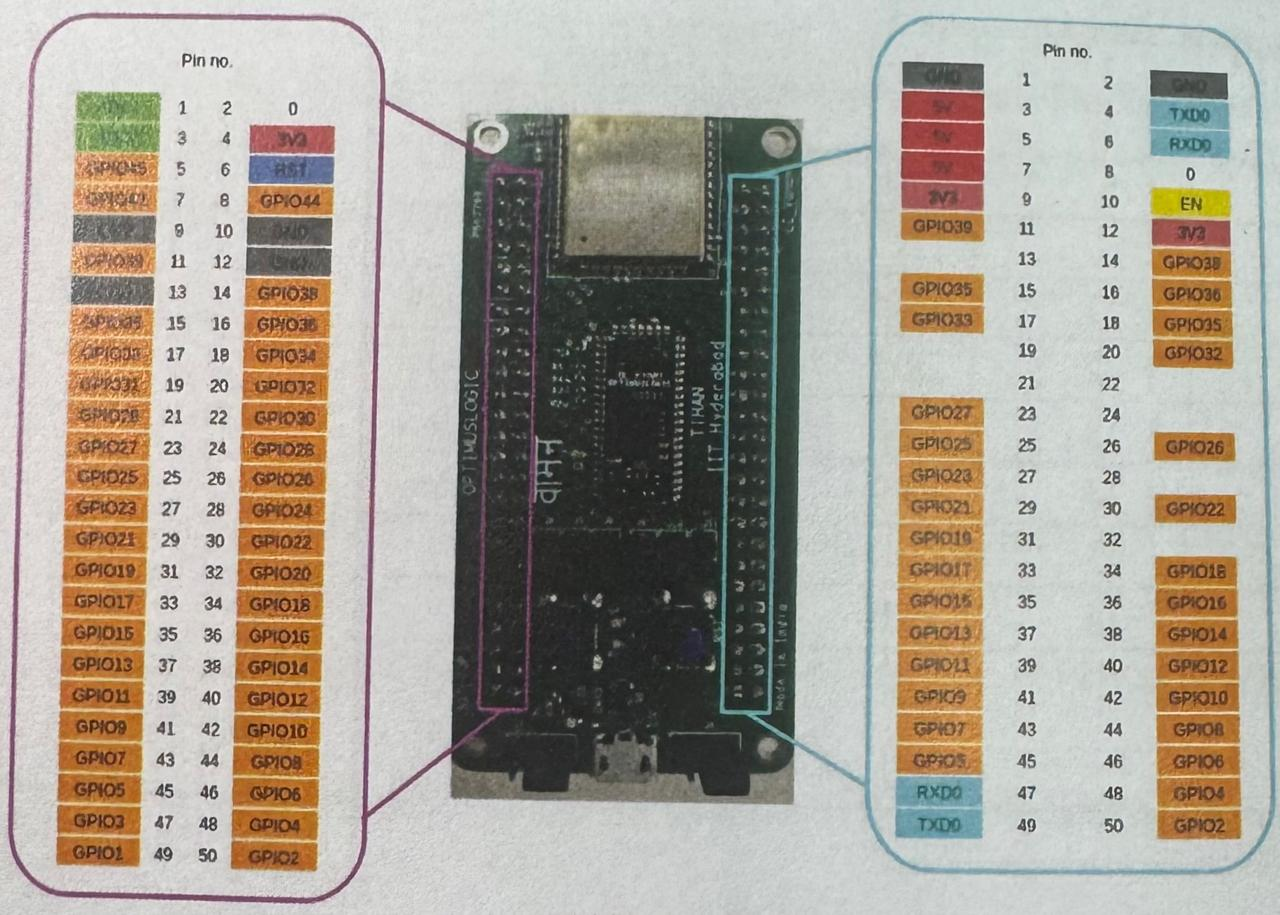
\includegraphics[width=0.4\textwidth]{vaman.jpg}       
\caption{\label{fig:1}}
 \end{figure}
 \begin{figure}[h]
 \centering
 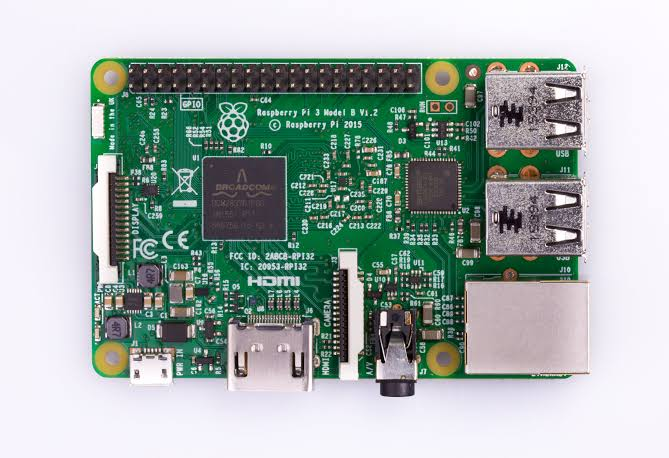
\includegraphics[width=0.4\textwidth]{piii.jpeg}
 \caption{\label{fig:1}}
 \end{figure}
\section{COMPONENTS}
The required components list is given in Table: I. 

 \begin{table} [htbp]
\centering
\begin{tabular}{| c | c | c |} \hline
Components & Value & Quantity \\\hline
LEDs &  & 1 \\ \hline
Vaman Board &  & 1 \\ \hline
Jumper Wires &  & 20 \\ \hline
	Raspberry pi 3 & & 1 \\ \hline
Breadboard & & 1 \\ 
\hline
\end{tabular}
\vspace{0.1cm}
\caption{\label{tab:widgets}}
\end{table}
\section{PROCEDURE}
 Connect the LED to GPIO pin 2 for output and D3, D2, D1 switches to GPIO pins 3, 4, and 5 (on Raspberry Pi) or pins 19, 20, 21 (on Vaman) as inputs. Ensure the inputs are connected to VCC or GND according to the truth table of the Boolean function. On the Raspberry Pi, use Python with the RPi.GPIO library to control the LED based on the inputs, while on the Vaman board, use the Arduino IDE to write code that reads the inputs and controls the LED. Finally, power on the board, run the respective program, and observe the LED behavior based on the simplified logic expression and observe the output based on the truth table.

\begin{table} [htbp]
\centering
\begin{tabular}{| c | c | c | c | c | c | c |} \hline
P & Q & R & S & $\bar{pq}$ & $\bar{qs}$ & F (P,Q,R,S)    \\\hline
0 & 0 & 0 & 0 & 1 & 1 & 1 \\ \hline
0 & 0 & 0 & 1 & 1 & 0 & 1 \\ \hline
0 & 0 & 1 & 0 & 1 & 1 & 1 \\ \hline
0 & 0 & 1 & 1 & 1 & 0 & 1 \\ \hline
0 & 1 & 0 & 0 & 0 & 1 & 1 \\ \hline
0 & 1 & 0 & 1 & 0 & 0 & 0 \\ \hline
0 & 1 & 1 & 0 & 0 & 1 & 1 \\ \hline
0 & 1 & 1 & 1 & 0 & 0 & 0 \\ \hline
1 & 0 & 0 & 0 & 0 & 1 & 1 \\ \hline
1 & 0 & 0 & 1 & 0 & 0 & 0 \\ \hline
1 & 0 & 1 & 0 & 0 & 1 & 1 \\ \hline
\end{tabular}
\vspace{0.2cm}
\caption{\label{tab:widgets}}
\end{table}

\section{RESULTS}
Download the code given in the link below and execute them to see the output. When the circuit is set up and the code is flashed through rasberry pi, the LED blinks according to the simplified Boolean function’s logic. Adjusting the inputs (D3, D2, and D1) as per the truth table causes the LED to turn on or off accordingly, validating the implementation of the simplified function.
https://github.com/salad-12/FWC-INTERNSHIP/blob/main/arm/code
\begin{figure}[h] 
 \centering 
 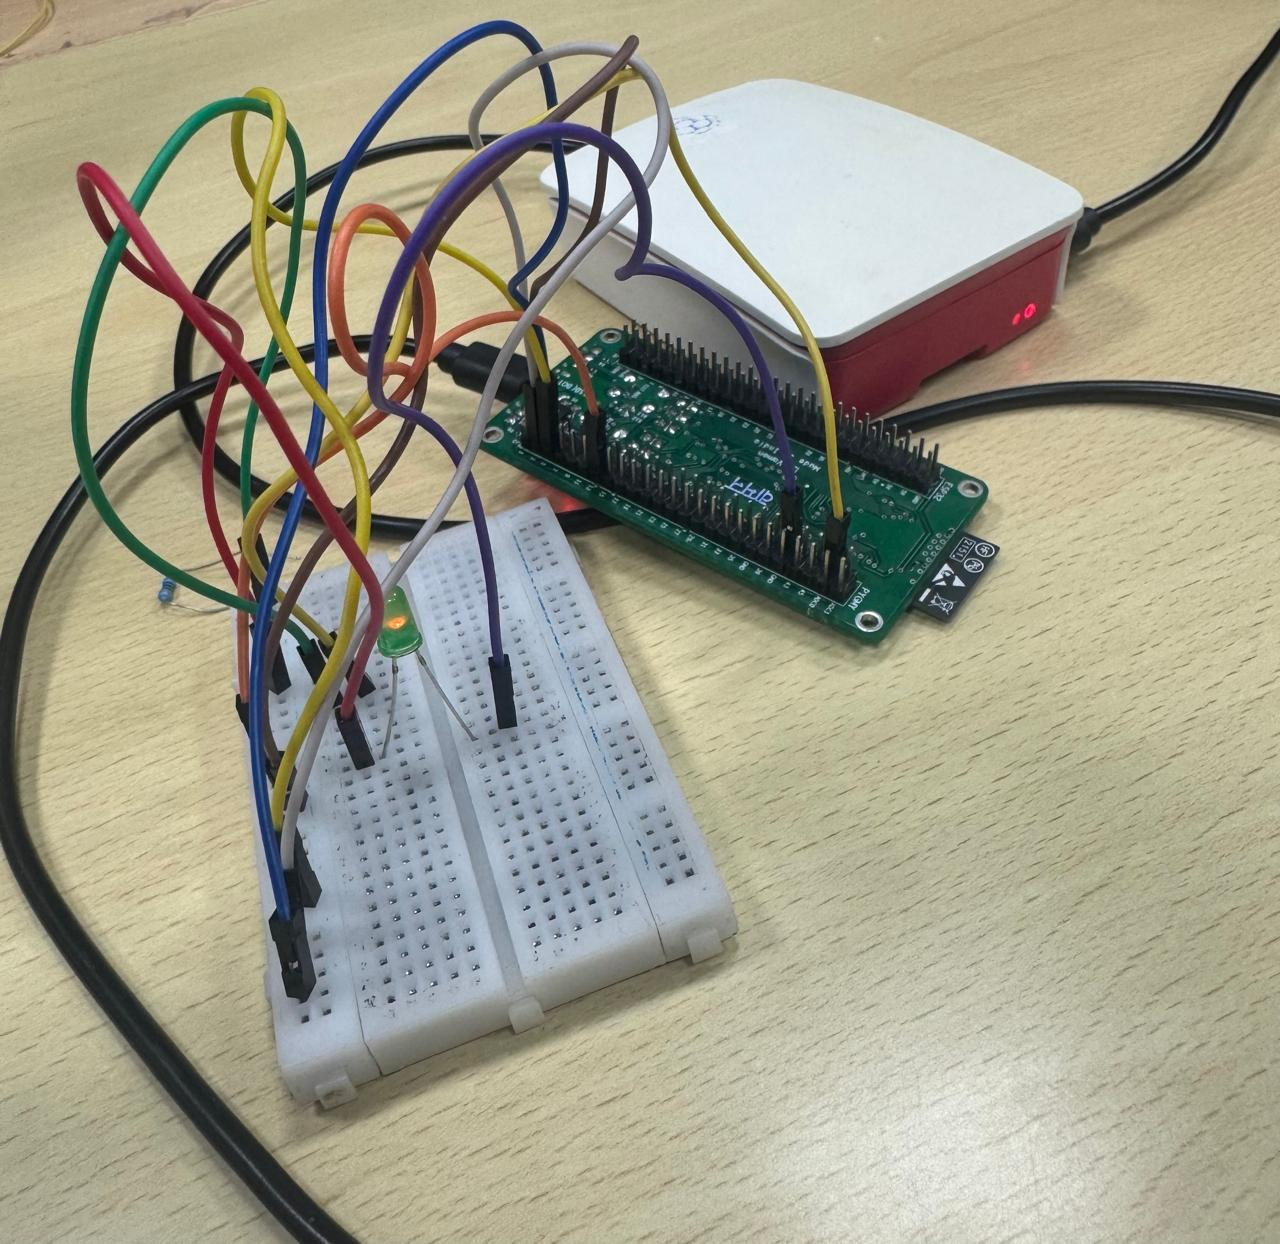
\includegraphics[width=0.4\textwidth]{arm.jpg}
 \caption{\label{fig:1}}    
\end{figure}
\section{CONCLUSION}
The experiment demonstrates the successful implementation of the simplified Boolean function using arm microcontroler through vaman board and raspberry pi. The LED’s behavior confirms the accuracy of the function's simplification, as it responds according to the specified truth table when the inputs are adjusted, verifying the logical operation and its hardware execution.
\end{document}
